% Figure 1, the conflict-aware calibration method. pdflatex fig_method; copy the PDF to ../figures.
\documentclass[tikz,border=3pt]{standalone}
\usepackage[T1]{fontenc}
\usepackage[scaled=0.92]{helvet}
\renewcommand{\familydefault}{\sfdefault}
\usepackage{amsmath,amssymb}
\usepackage{sansmath}
\sansmath
\DeclareRobustCommand{\sbarDelta}{\text{\fontencoding{OT1}\fontfamily{cmss}\fontseries{m}\fontshape{n}\selectfont\={\char1}}}
\usetikzlibrary{positioning,calc,arrows.meta,shadows.blur,backgrounds}

\definecolor{ink}{HTML}{1F2328}
\definecolor{ink2}{HTML}{57606A}
\definecolor{ink3}{HTML}{8C959F}
\definecolor{paper}{HTML}{F6F8FA}
\definecolor{cIn}{HTML}{57606A}
\definecolor{cA}{HTML}{0E7C86}
\definecolor{cB}{HTML}{2A78D6}
\definecolor{cC}{HTML}{E2662C}
\definecolor{cD}{HTML}{1A9E6F}
\definecolor{cOut}{HTML}{6E40C9}

\tikzset{
  badge/.style={circle, minimum size=1.95cm, line width=1.1pt, draw=#1, fill=#1!9,
                blur shadow={shadow blur steps=8, shadow xshift=0.5pt, shadow yshift=-0.8pt, shadow opacity=22}},
  num/.style={circle, fill=#1, text=white, font=\footnotesize\bfseries, inner sep=0pt, minimum size=0.46cm},
  title/.style={font=\normalsize\bfseries, text=#1!85!black},
  sub/.style={font=\footnotesize, text=ink2, align=center},
  flow/.style={-{Stealth[length=7pt,width=6pt]}, line width=1.4pt, color=ink3},
  chip/.style={rounded corners=3pt, draw=ink3!70, fill=white, inner sep=3pt, font=\footnotesize, text=ink, minimum height=0.62cm, align=left},
}

% ------------------------------------------------------------------ icons (drawn at origin, about 1.1 cm wide)
\newcommand{\icondiagnose}[1]{% matrix of pairs with a magnifying glass
  \foreach \i in {0,...,4} \foreach \j in {0,...,4} {
    \pgfmathtruncatemacro{\d}{abs(\i-\j)}
    \ifnum\d=1 \def\cc{cC!80}\else\ifnum\d=0 \def\cc{#1!45}\else\def\cc{#1!18}\fi\fi
    \fill[\cc] (-0.55+0.19*\i,0.4-0.19*\j) rectangle ++(0.16,-0.16);}
  \draw[ink, line width=1.6pt] (0.28,-0.18) circle (0.27);
  \fill[white, opacity=0.35] (0.28,-0.18) circle (0.26);
  \draw[ink, line width=2.4pt, line cap=round] (0.47,-0.37) -- (0.68,-0.58);}
\newcommand{\iconexplore}[1]{% population and Pareto front
  \draw[ink3, line width=0.6pt, -{Stealth[length=3pt]}] (-0.62,-0.5) -- (0.66,-0.5);
  \draw[ink3, line width=0.6pt, -{Stealth[length=3pt]}] (-0.62,-0.5) -- (-0.62,0.58);
  \foreach \p in {(-0.3,0.35),(-0.05,0.42),(0.2,0.22),(0.45,0.3),(0.1,0.05),(-0.25,0.12),(0.4,0.0),(0.55,0.42),(-0.42,0.45)}
    \fill[#1!45] \p circle (0.05);
  \draw[#1, line width=1.5pt] (-0.5,0.5) -- (-0.5,0.0) -- (-0.22,0.0) -- (-0.22,-0.2) -- (0.18,-0.2) -- (0.18,-0.33) -- (0.6,-0.33);
  \foreach \p in {(-0.5,0.0),(-0.22,-0.2),(0.18,-0.33)} \fill[#1] \p circle (0.065);}
\newcommand{\iconcertify}[1]{% shield with check mark
  \fill[#1] (0,0.6) .. controls (0.25,0.48) and (0.45,0.48) .. (0.55,0.45) -- (0.55,0.05)
        .. controls (0.55,-0.3) and (0.25,-0.52) .. (0,-0.62) .. controls (-0.25,-0.52) and (-0.55,-0.3) .. (-0.55,0.05)
        -- (-0.55,0.45) .. controls (-0.45,0.48) and (-0.25,0.48) .. (0,0.6) -- cycle;
  \draw[white, line width=2.6pt, line cap=round, line join=round] (-0.25,0.0) -- (-0.05,-0.2) -- (0.3,0.22);}
\newcommand{\iconselect}[1]{% front, budget line and target
  \draw[ink3, line width=0.6pt, -{Stealth[length=3pt]}] (-0.62,-0.5) -- (0.66,-0.5);
  \draw[ink3, line width=0.6pt, -{Stealth[length=3pt]}] (-0.62,-0.5) -- (-0.62,0.58);
  \draw[ink2, line width=1.2pt] (-0.5,0.5) -- (-0.5,0.08) -- (-0.15,0.08) -- (-0.15,-0.18) -- (0.3,-0.18) -- (0.3,-0.3) -- (0.6,-0.3);
  \draw[#1, line width=1pt, dash pattern=on 2.5pt off 1.5pt] (0.08,-0.5) -- (0.08,0.55);
  \draw[#1, line width=1.2pt] (-0.15,-0.18) circle (0.16);
  \draw[#1, line width=1pt] (-0.15,-0.18) circle (0.07);
  \draw[#1, line width=0.9pt] (-0.15,0.02) -- (-0.15,0.07) (-0.15,-0.38) -- (-0.15,-0.43) (-0.35,-0.18) -- (-0.4,-0.18) (0.05,-0.18) -- (0.1,-0.18);}
\newcommand{\iconoutput}[1]{% ranked list with check
  \foreach \k/\w in {0/1.0,1/0.8,2/0.62,3/0.48} {
    \fill[#1!80] (-0.55,0.42-0.27*\k) circle (0.075);
    \fill[#1!35, rounded corners=1.5pt] (-0.4,0.36-0.27*\k) rectangle ++(\w*0.95,0.12);}
  \fill[cD] (0.42,-0.36) circle (0.23);
  \draw[white, line width=1.8pt, line cap=round, line join=round] (0.31,-0.37) -- (0.39,-0.46) -- (0.54,-0.26);}
% input icons, small
\newcommand{\icontable}{%
  \draw[ink2, line width=0.7pt, rounded corners=1pt] (-0.22,-0.17) rectangle (0.22,0.17);
  \fill[ink2!35] (-0.22,0.08) rectangle (0.22,0.17);
  \draw[ink2, line width=0.5pt] (-0.22,-0.04) -- (0.22,-0.04) (-0.07,-0.17) -- (-0.07,0.17) (0.08,-0.17) -- (0.08,0.17);}
\newcommand{\iconscale}{%
  \draw[ink2, line width=0.8pt] (0,-0.17) -- (0,0.15) (-0.2,0.1) -- (0.2,0.14) (-0.1,-0.17) -- (0.1,-0.17);
  \draw[ink2, line width=0.6pt] (-0.2,0.1) -- (-0.27,-0.05) -- (-0.13,-0.05) -- cycle (0.2,0.14) -- (0.13,-0.01) -- (0.27,-0.01) -- cycle;}
\newcommand{\icongauge}{%
  \draw[ink2, line width=0.8pt] (-0.2,-0.08) arc (180:0:0.2);
  \draw[cC, line width=1.2pt] (-0.2,-0.08) arc (180:140:0.2);
  \draw[ink2, line width=0.8pt, -{Stealth[length=2pt]}] (0,-0.08) -- (-0.12,0.05);
  \fill[ink2] (0,-0.08) circle (0.03);}
% evaluation icons
\newcommand{\iconinsert}{\foreach \p in {(-0.15,0.06),(0.0,-0.08),(-0.05,0.12)} \fill[ink2] \p circle (0.035);
  \fill[cOut] (0.17,0.1) circle (0.04); \draw[cOut, line width=0.6pt, -{Stealth[length=2pt]}] (0.27,0.18) -- (0.2,0.12);}
\newcommand{\iconbars}{\fill[ink2!60] (-0.2,-0.12) rectangle ++(0.09,0.12) (-0.06,-0.12) rectangle ++(0.09,0.2) (0.08,-0.12) rectangle ++(0.09,0.08);
  \fill[cD] (0.22,-0.12) rectangle ++(0.09,0.28);}
\newcommand{\icondice}{\draw[ink2, line width=0.6pt, rounded corners=1.5pt] (-0.15,-0.15) rectangle (0.15,0.15);
  \foreach \p in {(-0.07,0.07),(0.07,-0.07),(0,0)} \fill[ink2] \p circle (0.03);}
\newcommand{\iconclock}{\draw[ink2, line width=0.7pt] (0,0) circle (0.15); \draw[ink2, line width=0.7pt] (0,0) -- (0,0.1) (0,0) -- (0.08,0);}

\begin{document}
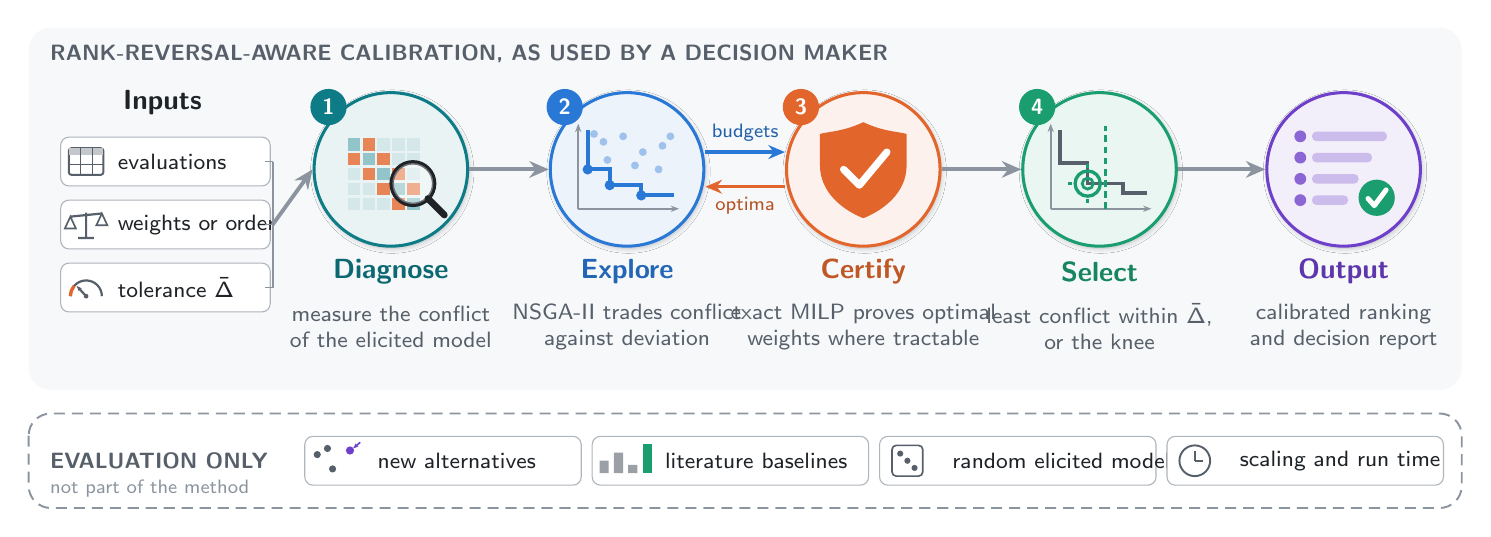
\begin{tikzpicture}[x=1cm,y=1cm]

% ---------------------------------------------------------------- method lane
\fill[paper, rounded corners=8pt] (-1.15,-2.05) rectangle (17.05,2.55);
\node[anchor=north west, font=\footnotesize\bfseries, text=ink2] at (-1.0,2.45) {RANK-REVERSAL-AWARE CALIBRATION, AS USED BY A DECISION MAKER};

% inputs
\node[font=\normalsize\bfseries, text=ink] at (0.55,1.6) {Inputs};
\node[chip, anchor=west] (i1) at (-0.75,0.85) {\makebox[2.45cm][l]{\hspace{0.62cm}evaluations}};
\node[chip, anchor=west] (i2) at (-0.75,0.05) {\makebox[2.45cm][l]{\hspace{0.62cm}weights or order}};
\node[chip, anchor=west] (i3) at (-0.75,-0.75) {\makebox[2.45cm][l]{\hspace{0.62cm}tolerance $\sbarDelta$}};
\begin{scope}[shift={(-0.42,0.85)}] \icontable \end{scope}
\begin{scope}[shift={(-0.42,0.05)}] \iconscale \end{scope}
\begin{scope}[shift={(-0.42,-0.78)}] \icongauge \end{scope}

% stage badges
\foreach \x/\c/\n/\name in {3.45/cA/1/A, 6.45/cB/2/B, 9.45/cC/3/C, 12.45/cD/4/D} {
  \node[badge=\c] (b\name) at (\x,0.75) {};
  \node[num=\c] at ($(b\name)+(135:1.12)$) {\n};
}
\begin{scope}[shift={(bA)}] \icondiagnose{cA} \end{scope}
\begin{scope}[shift={(bB)}] \iconexplore{cB} \end{scope}
\begin{scope}[shift={(bC)}] \iconcertify{cC} \end{scope}
\begin{scope}[shift={(bD)}] \iconselect{cD} \end{scope}

\node[title=cA] at (3.45,-0.55) {Diagnose};
\node[sub] at (3.45,-1.25) {measure the conflict\\of the elicited model};
\node[title=cB] at (6.45,-0.55) {Explore};
\node[sub] at (6.45,-1.25) {NSGA-II trades conflict\\against deviation};
\node[title=cC] at (9.45,-0.55) {Certify};
\node[sub] at (9.45,-1.25) {exact MILP proves optimal\\weights where tractable};
\node[title=cD] at (12.45,-0.55) {Select};
\node[sub] at (12.45,-1.25) {least conflict within $\sbarDelta$,\\or the knee};

% output
\node[badge=cOut] (bO) at (15.55,0.75) {};
\begin{scope}[shift={(bO)}] \iconoutput{cOut} \end{scope}
\node[title=cOut] at (15.55,-0.55) {Output};
\node[sub] at (15.55,-1.25) {calibrated ranking\\and decision report};

% flows
\draw[flow] (1.95,0.05) -- (bA.west);
\draw[flow] (bA.east) -- (bB.west);
\draw[flow] (bC.east) -- (bD.west);
\draw[flow] (bD.east) -- (bO.west);
\draw[-{Stealth[length=6pt,width=5pt]}, line width=1.2pt, cB] ($(bB.east)+(0,0.22)$) -- node[above, font=\scriptsize, text=cB!80!black] {budgets} ($(bC.west)+(0,0.22)$);
\draw[-{Stealth[length=6pt,width=5pt]}, line width=1.2pt, cC] ($(bC.west)+(0,-0.22)$) -- node[below, font=\scriptsize, text=cC!80!black] {optima} ($(bB.east)+(0,-0.22)$);
\draw[ink3, line width=0.6pt] (1.95,0.85) -- (1.95,-0.75);
\draw[ink3, line width=0.6pt] (1.85,0.85) -- (1.95,0.85) (1.85,0.05) -- (1.95,0.05) (1.85,-0.75) -- (1.95,-0.75);

% ---------------------------------------------------------------- evaluation lane
\draw[ink3, rounded corners=8pt, dash pattern=on 4pt off 2.5pt, line width=0.7pt] (-1.15,-2.35) rectangle (17.05,-3.55);
\node[anchor=west, font=\footnotesize\bfseries, text=ink2] at (-1.0,-2.95) {EVALUATION ONLY};
\node[anchor=west, font=\scriptsize, text=ink3, align=left] at (-1.0,-3.3) {not part of the method};
\foreach \x/\ic/\txt in {2.35/\iconinsert/new alternatives, 6.0/\iconbars/literature baselines, 9.65/\icondice/random elicited models, 13.3/\iconclock/scaling and run time} {
  \node[chip, anchor=west] at (\x,-2.95) {\makebox[3.3cm][l]{\hspace{0.82cm}\txt}};
  \begin{scope}[shift={(\x+0.36,-2.95)}, scale=1.3] \ic \end{scope}
}
\end{tikzpicture}
\end{document}
